% id: 130-c5
% book: 개념원리 중학 3-2 · 13 상자그림
% section: 핵심문제 익히기
% figure: crop:fig-130-c5.png
% answer: ⑴ 16시간, 18시간 ⑵ $\pt{B}$ 건전지
% answer_source: 답지
% variant_level: 0 (원본 전사)
% 이 파일은 build.mjs 가 items.json 에서 만든다. 고칠 때는 items.json 을 고친다.
\smash{\raisebox{1.5mm}{\dmkichul{개념원리 중학 3-2 130쪽 확인 5}}}
오른쪽 그림은 같은 기기에서 $\pt{A}$, $\pt{B}$ 두 건전지의 수명을 조사하여 나타낸 상자그림이다. 다음 물음에 답하시오.
\par\smallskip\begin{center}\setlength{\dmfigw}{181.1pt}\ifdim\dmfigw>\linewidth\setlength{\dmfigw}{\linewidth}\fi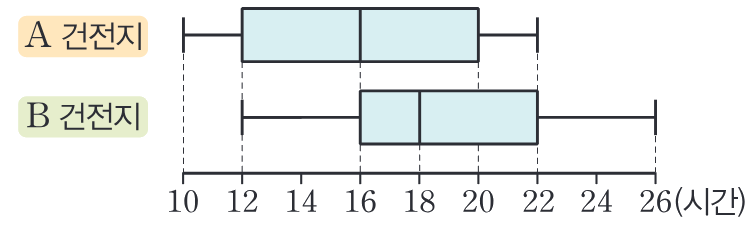
\includegraphics[width=\dmfigw]{figures/fig-130-c5.png}\end{center}
\dmsubprob{1} $\pt{A}$, $\pt{B}$ 두 건전지의 수명의 중앙값을 차례대로 구하시오.
\dmsubprob{2} $\pt{A}$, $\pt{B}$ 두 건전지 중 어느 건전지를 사용하는 것이 더 유리한지 구하시오.
